\documentclass[../main.tex]{subfiles}
\addbibresource{../bibfile.bib}

\begin{document}

\chapter{Metodologie utilizzate}
\label{chap:oth}
Questo capitolo è dedicato all'esposizione delle diverse metodologie statiche e dinamiche alla base delle tecniche di analisi rese disponibili dalla piattaforma.
In particolare, verranno illustrati i concetti teorici alla loro base e verranno forniti esempi per illustrarne il funzionamento su casi concreti.
\section{Disassembling}
Generalmente, la catena di compilazione di un linguaggio ad alto livello prevede una fase di \textit{assemblaggio}, in cui il codice assembly generato dal compilatore viene tradotto
nel linguaggio macchina specifico dell'architettura della CPU su cui il programma dovrà essere eseguito. Questa traduzione stabilisce quindi una relazione uno-a-uno tra le istruzioni macchina
prodotte dall'\textit{assemblatore} e le istruzioni assembly definita dalla \textit{Instruction Set Architecture} (ISA) dell'architettura del processore.
Questa relazione permette di effettuare anche la traduzione inversa e recuperare il codice assembly dall'insieme di istruzioni macchina presenti in un file binario.
Questo processo è noto con il nome di \textbf{disassembling}. Effettuare il disassembly di un programma è una pratica fondamentale nell'ambito del reverse engineering, poiché permette di analizzare, in un formato leggibile dall'essere umano (assembly), le operazioni
di basso livello che verranno eseguite dal calcolatore, rendendo possibile l'individuazione di potenziali problematiche di sicurezza sfruttabili da un attaccante.
Seppur sembri un processo relativamente semplice, effettuare il disassembly di un codice macchina richiede di gestire diverse problematiche \cite{Disassembly2}:
\begin{itemize}
    \item \textbf{Jump tables}: una \textit{jump-table} è un array di indirizzi comunemente usata per per implementare trasferimenti del flusso di controllo multi-direzionali (ad esempio, la trasposizione a basso livello del costrutto \textit{switch} del linguaggio \textit{C}).
    L'idea alla base dell'utilizzo di una jump table è quella di recuperare l'indirizzo a cui saltare indicizzando l'array con il valore dell'espressione per poi effettuare un jump indiretto verso l'indirizzo recuperato.
    Il codice che si occupa di questo processo è di solito preceduto da un controllo sul valore dell'espressione (\textit{bound check}) per assicurarsi che non si stia cercando di accedere ad un indice non presente nell'array.
    Un disassembler dovrà quindi necessariamente stimare correttamente la grandezza della jump table per garantire la qualità del disassembly prodotto.
    \item \textbf{Position-Independent Code (PIC)}: Molti compilatori generano codice che può essere caricato ed eseguito indipendentemente dalla specifica sezione dello spazio di indirizzamento in cui vene caricato il programma.
    Questo tipo di codice viene detto \textit{Position-Independent Code} (PIC). Quando viene prodotto PIC, il compilatore tipicamente crea delle \textit{jump tables}, anch'esse indipendenti dalla posizione e formate da una serie di offset, le quali vengono inserite all'interno della sezione dell'eseguibile dedicata al codice (la "\textit{text}" section).
    L'offset presente all'interno di queste tabelle verrà poi sommato all'indirizzo caricato al momento pe raggiungere la posizione desiderata tramite un jump indiretto.
    La presenza di PIC introduce due criticità che complicano il processo di disassembly:
    \begin{itemize}
        \item Le tabelle sono \textbf{indistinguibili dai dati presenti nell'eseguibile}
        \item Le sezioni di codice che effettuano i jump indiretti sono spesso \textbf{complesse} e non aderiscono a pattern di codice facilmente riconoscibili
    \end{itemize}
    Considerate insieme, queste caratteristiche rendono il disassembly di sequenze di PIC contenenti jump table più problematiche rispetto all'analisi di codice standard.
\end{itemize}
\section{Control Flow Graph (CFG)}
Considerare adeguatamente il flusso di controllo di un programma, cioè quali istruzioni vengono eseguite dato un certo input, è fondamentale per effettuare un'analisi di sicurezza accurata. Risulterebbe infatti inutile segnalare
una problematica di sicurezza data da un segmento irraggiungibile del codice di un programma. Vorremmo quindi un modo per rappresentare tutti i possibili cammini di esecuzione che un programma può intraprendere.
Per farlo, possiamo possiamo basarci sulle seguenti definizioni: chiameremo \textit{basic block} una \textbf{sequenza massimale contigua di statement del programma}. Allora, un \textit{Control-Flow Graph (CFG)} per un programma $P$ è un grafo $G$ diretto e orientato dove:
\begin{itemize}
    \item I nodi di $G$ sono i basic block di $P$
    \item Gli archi di $G$ connettono i basic block che sono in una relazione di sequenza (uno segue l'altro). Gli archi possono etichettati con "true" o "false" se il basic block sorgente termina con un controllo condizionale 
\end{itemize}
Durante la costruzione di un CFG, è importante gestire correttamente le istruzioni condizionali \textit{if} e \textit{while}:
\begin{itemize}
    \item \textbf{If}: Il controllo condizionale termina il basic block a cui appartiene lo statement precedente. Due archi etichettati rispettivamente con "true" e "false" connettono il basic
    block in cui è contenuta l'istruzione \textit{if} ai basic block rispettivamente dei rami "then" e "else". La fine dei basic block dei rami "then" ed "else" hanno archi non etichettati
    verso il basic block degli statement che seguono l’"if" statement
    \item \textbf{While}: Questo tipo di statement crea un \textbf{basic block a se stante}, il quale avrà due archi uscenti etichettati rispettivamente "true", verso il
    basic block del corpo del ciclo, e "false", verso il basic block degli statement dopo il ciclo
\end{itemize}
\newpage \noindent
Supponiamo, per esempio, di avere il seguente programma:
\lstinputlisting[language=C, caption = Un programma in C che calcola il massimo numero in un array di cinque elementi, firstline = 3]{../code_examples/exemple1.c}
Allora, il suo CFG sarà: \newline
\begin{figure}[H]
    \centering
    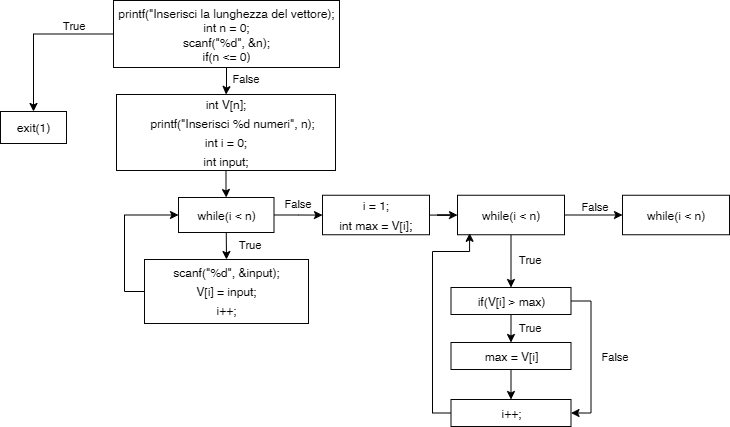
\includegraphics[width = 1\linewidth]{../images/CFG.drawio.png}
    \caption{CFG del programma illustrato nel listing 3.1}
\end{figure}




\section{Decompiling}
Dato un programma binario, è possibile \textbf{ricostruire il codice ad alto livello} in cui è stato scritto attraverso un processo noto come \textit{decompiling}.
Lo scopo di un \textit{decompiler} (o \textit{reverse compiler}) è quindi quello di recuperare, partendo dal codice macchina, un programma scritto in un linguaggio ad alto livello che effettua le stesse
operazioni del programma binario dato in input \cite{Cifuentes1995DecompilationOB}.








\end{document}